\documentclass[UTF8]{ctexart}
\usepackage{graphicx}
\graphicspath{{img/}} 
\title{Homework\ 3}
\author{PB17111623}
\author{PB17111623 范睿}
\date{\today}
\usepackage[a4paper,bottom=3.5cm]{geometry}
\usepackage{algorithm}  
\usepackage{algorithmicx}
\usepackage{amsmath}  
\usepackage{algpseudocode}  %算法的包
\usepackage{amssymb}
\begin{document}
\maketitle
\section{HW3}
\subsection{证明:包含 n 个元素的堆的 Max-Heapify 函数的时间复杂度是$\mathcal{O}(\log n)$,Build-Max-Heap 函数的时间复杂度是 $\mathcal{O}(n)$}
证明:\\
在最坏情况下,每一次调用Max-Heapify函数都会进入“if largest $\neq$ i”的条件中。第一次调用Max-Heapify时,向算法传递的第二个参数i为A.length/2,即有子节点的节点中下标最大结点的下标。在最坏情况下,每一次调用向Max-Heapify传递的第二个参数i沿着二叉树的结点一直到 根结点1结束。因此在最坏情况下,算法的复杂度为此树的高度。由于包含n个元素的完全二叉树的高度为$\log n$,Max-Heapify的复杂度为$\mathcal{O}(\log n)$。
\\\\在一个高度为$h$的结点上运行MAX-HEAPIFY的代价是$\mathcal(O)(h)$,则总代价为\\
\begin{equation*}
\sum_{h=0}^{\lfloor \lg n\rfloor}\lceil \frac{n}{2^{h+1}}\rceil \mathcal O(h) = \mathcal O(n \sum_{h=0}^{\lfloor \lg n \rfloor}\frac{h}{2^h})
\end{equation*}
有\\
\begin{equation*}
\sum_{h=0}^\infty \frac{h}{2^h}=2
\end{equation*}
则
\begin{equation*}
\mathcal O(n \sum_{h=0}^{\lfloor \lg n \rfloor}\frac{h}{2^h}) = \mathcal O(n \sum_{h=0}^{\infty}\frac{h}{2^h})=\mathcal O(n)
\end{equation*}
综上,Build-Max-Heap的时间复杂度为$\mathcal O(n)$
\subsection{试证明:在一个随机输入数组上,对于任何常数 $0 \textless \alpha \leq \frac{1}{2}$,Partition 产生比 $1-\alpha : \alpha$  更平衡的划分的概率约为 $1 - 2\alpha$}
证明:\\\\
\centerline{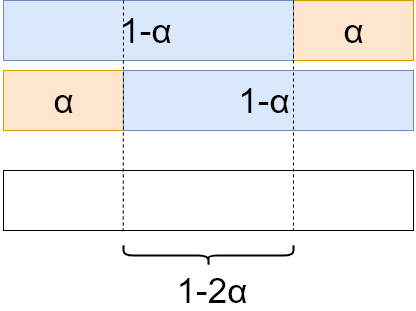
\includegraphics[scale=0.5]{img/2.png}}
如图所示,产生$1- \alpha:\alpha$的划分比例的情况可能为前两排两种,即$\alpha$部分在最左和最右。那么比$1- \alpha:\alpha$更平均的分割就是分割线在第三行被扩起来的部分。由于输入随机,因此更平均的概率为$1- 2\alpha$。

\subsection{假设快速排序的每一层所做的划分比例都是 $1-\alpha : \alpha$,其中 $0 \textless \alpha \leq \frac{1}{2}$ 且是一个常数. 试证明:在相应的递归树中,叶结点的最小深度大约是 $- \frac{\lg n}{\lg \alpha}$,最大深度大约是 $- \frac{\lg n}{\lg (1− \alpha)}$(无需考虑舍入问题).}
我们可以沿着每一层$1- \alpha$的划分分支寻找到最深的叶结点,因此\\
\centerline{$(1- \alpha)^{h_{max}}n=1$}
\centerline{$h_{max}=\log_{1- \alpha}{\frac{1}{n}}$}
\centerline{$h_{max}=\frac{\lg \frac{1}{n}}{\lg (1- \alpha)}$}
\centerline{$h_{max}=-  \frac{\lg n}{\lg (1- \alpha)}$}
同理,沿着每一层$\alpha$的划分可以找到最浅的叶结点,有\\
\centerline{$\alpha^{h_{min}}n=1$}
\centerline{$h_{min}=\log_{\alpha}{\frac{1}{n}}$}
\centerline{$h_{min}=-\frac{\lg n}{\lg \alpha}$}
\end{document}